\documentclass[11pt, a4paper]{article}
\usepackage[utf8]{inputenc}\usepackage[spanish, es-tabla]{babel}
\usepackage{geometry}
\geometry{top=2.5cm, bottom=2.5cm, left=2.5cm, right=2.5cm}
\usepackage{amsmath, amsfonts, amssymb}
\usepackage{graphicx}
\usepackage{booktabs}
\usepackage{multirow}
\usepackage{tabularx}
\usepackage{hyperref}
\usepackage{cite}

\hypersetup{
    colorlinks=true,
    linkcolor=blue,
    citecolor=blue,
    urlcolor=blue
}

\title{\textbf{IEEE 29148:2018 y Tipos de Requisitos en un Sistema Conocido (Duolingo)} \\ }
\author{\textbf{Frixon Moran} \\ Universidad Técnica Estatal de Quevedo \\ Facultad de Ciencias de la Computación \\ Carrera de Software --- 4.º Nivel Paralelo A \\ \texttt{fmoranp@uteq.edu.ec}}
\date{}

\begin{document}

\maketitle

\begin{abstract}
El presente documento analiza la aplicación de la norma ISO/IEC/IEEE 29148:2018 y el modelo de calidad del producto ISO/IEC 25010:2023 en el contexto del sistema de aprendizaje de idiomas gamificado \textbf{Duolingo}. Se desarrolla un resumen analítico detallado de la norma, un glosario conceptual basado en su Cláusula 3, la especificación formal de 15 requisitos clasificados por tipo y cuantificados con métricas objetivas, un proceso de autoevaluación estricto contra las directrices de la norma y una reflexión crítica sobre el proceso de especificación.
\end{abstract}

\section{Descripción del Sistema Seleccionado}
El sistema seleccionado para el desarrollo de esta actividad es \textbf{Duolingo}, una plataforma multiplataforma (móvil y web) orientada al aprendizaje gamificado de idiomas mediante lecciones interactivas de corta duración. 
\begin{itemize}
    \item \textbf{Propósito:} Facilitar la adquisición de habilidades lingüísticas autónomas mediante mecánicas de juego (puntos de experiencia, rachas diarias, ligas competitivas y vidas/corazones).
    \item \textbf{Usuarios:} Estudiantes, profesionales y público general de cualquier rango etario con interés en aprender o reforzar un nuevo idioma.
    \item \textbf{Contexto de operación:} Operación en entornos móviles (Android/iOS) y navegadores web con conexión intermitente o continua a Internet, requiriendo sincronización en tiempo real de estados de usuario y datos de progreso.
\end{itemize}

\section{Resumen Analítico: ISO/IEC/IEEE 29148:2018}

\subsection{El Requisito Bien Formado}
La norma ISO/IEC/IEEE 29148:2018 establece en su Cláusula 5.2.4 que un requisito bien formado es una declaración verbal o sintáctica formal que expresa una necesidad, condición o capacidad que el sistema debe satisfacer de forma inequívoca \cite{iso29148}. Un requisito no debe describir diseño ni implementación, sino la capacidad verificable requerida por el adquirente o usuario. La norma enfatiza el uso de construcciones gramaticales estrictas basadas en la fórmula: \textit{Condición + Sujeto + Verbo Imperativo (debe/shall) + Acción + Restricción/Métrica}.

\subsection{Características de un Requisito Individual}
De acuerdo con la Cláusula 5.2.5, cada requisito de manera individual debe poseer las siguientes nueve características indispensables \cite{iso29148}:
\begin{enumerate}
    \item \textbf{Necesario:} Define una capacidad indispensable sin la cual el sistema no satisface la necesidad real de los stakeholders.
    \item \textbf{Imperativo:} Declara qué debe hacer el sistema sin imponer soluciones técnicas o de diseño prematuras.
    \item \textbf{No ambiguo:} Admite una sola interpretación objetiva por parte de desarrolladores, evaluadores y usuarios.
    \item \textbf{Completo:} Contiene toda la información necesaria sin requerir explicaciones adicionales para su comprensión.
    \item \textbf{Singular:} Expresa una sola necesidad o capacidad del sistema, evitando conjunciones que agrupen múltiples funciones.
    \item \textbf{Realizable:} Puede ser implementado dentro de los límites técnicos, presupuestarios y temporales del proyecto.
    \item \textbf{Verificable:} Existe un método objetivo (prueba, inspección, análisis o demostración) para comprobar su cumplimiento.
    \item \textbf{Conforme:} Sigue la sintaxis, estructura y normas acordadas para la redacción de requerimientos.
    \item \textbf{Modificable:} Su estructura permite cambios posteriores sin impactar de forma desproporcionada otros requerimientos.
\end{enumerate}

\subsection{Características del Conjunto de Requisitos}
A nivel colectivo, la Cláusula 5.2.6 dicta que el conjunto de requisitos debe exhibir las propiedades de completitud (no faltan elementos funcionales o de calidad), consistencia (inexistencia de contradicciones internas o incompatibilidades), factibilidad general y trazabilidad (capacidad de rastrear el origen y evolución de cada enunciado) \cite{iso29148}.

\subsection{Términos Ambiguos Prohibidos}
La Cláusula 5.2.7 prohíbe explícitamente el uso de vocabulario vago o subjetivo que impida la verificación objetiva \cite{iso29148}. Entre los términos restringidos se encuentran: \textit{user-friendly} (fácil de usar), \textit{fast} (rápido), \textit{robust} (robusto), \textit{efficient} (eficiente), \textit{adequate} (adecuado), \textit{state-of-the-art} (de última generación), \textit{as far as possible} (en la medida de lo posible) y adverbios temporales ambiguos como \textit{pronto} o \textit{inmediatamente}.

\section{Glosario de Términos}
A continuación se definen 10 términos clave extrapolados de la Cláusula 3 de la norma ISO/IEC/IEEE 29148:2018 \cite{iso29148}, aplicados al contexto operativo de Duolingo:

\begin{enumerate}
    \item \textbf{Adquirente:} Entidad o individuo que adquiere un sistema o servicio. \textit{Ejemplo en Duolingo:} Un usuario que compra la suscripción premium "Super Duolingo".
    \item \textbf{Línea Base:} Versión formalmente aprobada de un artefacto que sirve de referencia para desarrollos futuros. \textit{Ejemplo en Duolingo:} La especificación aprobada para el algoritmo de aprendizaje adaptativo versión 4.2.
    \item \textbf{Cliente:} Parte que recibe el producto o servicio final. \textit{Ejemplo en Duolingo:} El estudiante que interactúa a diario con los módulos de vocabulario.
    \item \textbf{Stakeholder:} Persona u organización que tiene derechos o intereses en el sistema. \textit{Ejemplo en Duolingo:} Diseñadores instruccionales, ingenieros backend y usuarios finales.
    \item \textbf{Requisito:} Condición o capacidad necesaria para resolver un problema o lograr un objetivo. \textit{Ejemplo en Duolingo:} La capacidad del sistema de descontar vidas al cometer un error gramatical.
    \item \textbf{Verificación:} Confirmación mediante evidencia de que se han cumplido los requisitos especificados. \textit{Ejemplo en Duolingo:} Ejecución de pruebas automatizadas para comprobar el tiempo de carga de las lecciones.
    \item \textbf{Validación:} Confirmación de que el sistema cumple con el uso previsto en su entorno real. \textit{Ejemplo en Duolingo:} Evaluación empírica del retención de vocabulario en usuarios reales.
    \item \textbf{Concepto de Operaciones:} Descripción del funcionamiento del sistema desde la perspectiva del usuario. \textit{Ejemplo en Duolingo:} El flujo operativo desde que el usuario inicia sesión hasta completar la racha diaria.
    \item \textbf{Modificabilidad:} Capacidad del sistema para incorporar cambios sin degradar su estructura. \textit{Ejemplo en Duolingo:} Facilidad para añadir una nueva rama de idioma en el árbol de lecciones.
    \item \textbf{Calidad:} Grado en que un conjunto de características inherentes cumple con los requisitos expuestos. \textit{Ejemplo en Duolingo:} El porcentaje de disponibilidad del servicio de sincronización en la nube ($>99.9\%$).
\end{enumerate}

\section{Formulación de Requisitos del Sistema}
Se especifican 15 requisitos del sistema Duolingo abarcando 5 tipos distintos según la norma ISO/IEC/IEEE 29148 \cite{iso29148}. Los 5 primeros corresponden a requisitos de calidad (no funcionales) clasificados formalmente con el estándar ISO/IEC 25010:2023 \cite{iso25010}.

\subsection{Requisitos de Calidad}
\begin{itemize}
    \item \textbf{RF-CAL-01 (Eficiencia de desempeño / Comportamiento temporal):} El servidor backend de Duolingo debe responder a la petición HTTP de registro de XP al finalizar una lección en un tiempo inferior o igual a 1.5 segundos bajo conexiones 4G.
    \item \textbf{RF-CAL-02 (Fiabilidad / Madurez):} La aplicación móvil de Duolingo no debe presentar cierres imprevistos (\textit{crashes}) en más del 0.1\% de las sesiones activas diarias de estudio.
    \item \textbf{RF-CAL-03 (Seguridad / Confidencialidad):} El sistema debe cifrar las contraseñas de los usuarios guardadas en la base de datos utilizando el algoritmo bcrypt con un factor de trabajo (\textit{cost factor}) mayor o igual a 12.
    \item \textbf{RF-CAL-04 (Usabilidad / Reconocibilidad de la adecuación):} El 95\% de los usuarios nuevos identificará el botón "Empezar Lección" en un tiempo menor a 4 segundos durante la primera sesión de uso.
    \item \textbf{RF-CAL-05 (Mantenibilidad / Modificabilidad):} El sistema debe permitir la adición de nuevos conjuntos de frases en formato JSON en el repositorio sin requerir la recompilación del binario ejecutable móvil.
\end{itemize}

\subsection{Requisitos Funcionales (RF)}
\begin{itemize}
    \item \textbf{RF-06:} El sistema debe sustraer exactamente 1 corazón de la cuenta del usuario cuando este confirme una respuesta incorrecta en un ejercicio.
    \item \textbf{RF-07:} El sistema debe incrementar en 1 unidad la racha diaria del usuario al completar al menos 1 lección completa antes de las 23:59 horas locales.
    \item \textbf{RF-08:} El sistema debe emitir una notificación emergente (\textit{push}) a las 20:00 horas si el usuario no registra actividad de estudio en el día en curso.
    \item \textbf{RF-09:} El sistema debe permitir la recuperación de acceso enviando un enlace tokenizado de un solo uso al correo electrónico registrado.
\end{itemize}

\subsection{Requisitos de Desempeño (RD)}
\begin{itemize}
    \item \textbf{RD-10:} La infraestructura debe procesar hasta 40,000 peticiones concurrentes por segundo durante las horas pico de tráfico sin exceder un tiempo de respuesta de 2.0 segundos.
    \item \textbf{RD-11:} El paquete de datos descargable de una lección offline de idioma no debe superar un tamaño total de 15 MB.
\end{itemize}

\subsection{Requisitos de Interfaz Externa (RIE)}
\begin{itemize}
    \item \textbf{RIE-12:} La interfaz del cliente móvil debe adaptarse automáticamente a pantallas con resoluciones desde $720 \times 1280$ píxeles hasta $1440 \times 3200$ píxeles manteniendo la legibilidad del texto.
    \item \textbf{RIET-13:} El sistema debe conectarse con la API de Google Play Billing para procesar pagos y validar el estado de las suscripciones.
\end{itemize}

\subsection{Restricciones (RES)}
\begin{itemize}
    \item \textbf{RES-14:} El microservicio de recomendaciones interactivas debe ejecutarse en contenedores Docker gestionados en entornos de Amazon Web Services.
    \item \textbf{RES-15:} La gestión de los datos personales de los usuarios en Ecuador debe ceñirse a las disposiciones de la Ley Orgánica de Protección de Datos Personales (LOPDP) \cite{lopdp2021}.
\end{itemize}

\section{Tabla de Clasificación y Criterios de Aceptación}
La Tabla \ref{tab:clasificacion} sintetiza los requisitos formulados, sus métricas cuantificables y sus criterios de aceptación.

\begin{table}[htbp]
\centering
\caption{Clasificación de requisitos, métricas y criterios de aceptación.}
\label{tab:clasificacion}
\small
\begin{tabularx}{\textwidth}{l X l X X}
\toprule
\textbf{ID} & \textbf{Enunciado Resumido} & \textbf{Tipo} & \textbf{Métrica} & \textbf{Criterio de Aceptación} \\
\midrule
RF-CAL-01 & Latencia registro XP & Calidad (ISO 25010) & Tiempo de respuesta en ms & $\le 1500$ ms en el 99\% de las peticiones. \\
RF-CAL-02 & Tasa de cierres fallidos & Calidad (ISO 25010) & \% cierres por sesión & $< 0.1\%$ de fallos por 10,000 sesiones. \\
RF-CAL-03 & Cifrado de claves & Calidad (ISO 25010) & Algoritmo y coste & Bcrypt con coste $\ge 12$ verificado. \\
RF-CAL-04 & Usabilidad en inicio & Calidad (ISO 25010) & Tiempo de detección & $\ge 95\%$ usuarios ubican botón en $< 4$ s. \\
RF-CAL-05 & Despliegue de frases & Calidad (ISO 25010) & Tiempo de actualización & Actualización JSON sin compilar ejecutable. \\
RF-06 & Resta de corazones & Funcional & Conteo de vidas & Reducción exacta de $N$ a $N-1$ por error. \\
RF-07 & Incremento de racha & Funcional & Contador de días & Incremento $+1$ al completar lección. \\
RF-08 & Notificación push & Funcional & Hora de envío & Emisión del mensaje a las 20:00 exactas. \\
RF-09 & Reseteo clave & Funcional & Envío de correo & Enlace temporal enviado en $< 30$ s. \\
RD-10 & Peticiones concurrentes & Desempeño & Solicitudes / segundo & Support 40,000 req/s con error HTTP $< 0.01\%$. \\
RD-11 & Peso de lección & Desempeño & Megabytes (MB) & Archivo descargado $\le 15$ MB. \\
RIE-12 & Adaptabilidad pantalla & Interfaz Externa & Rango de resolución & Despliegue sin solapamientos ($720\text{p}$ a $1440\text{p}$). \\
RIE-13 & Pasarela de pago & Interfaz Externa & Respuesta Google API & Transacción validada correctamente vía webhook. \\
RES-14 & Contenedores Docker & Restricción & Imagen desplegada & Ejecución completa sobre infraestructura AWS. \\
RES-15 & Cumplimiento LOPDP & Restricción & Auditoría de datos & Consentimiento y revocación según norma \cite{lopdp2021}. \\
\bottomrule
\end{tabularx}
\end{table}

\section{Evidencias del Sistema (Capturas de Pantalla)}
Las Figuras \ref{fig:duolingo1}, \ref{fig:duolingo2} y \ref{fig:duolingo3} muestran las evidencias operativas extraídas de la aplicación Duolingo, las cuales respaldan la formulación de los requisitos funcionales y de usabilidad especificados en este informe.

\begin{figure}[htbp]
    \centering
    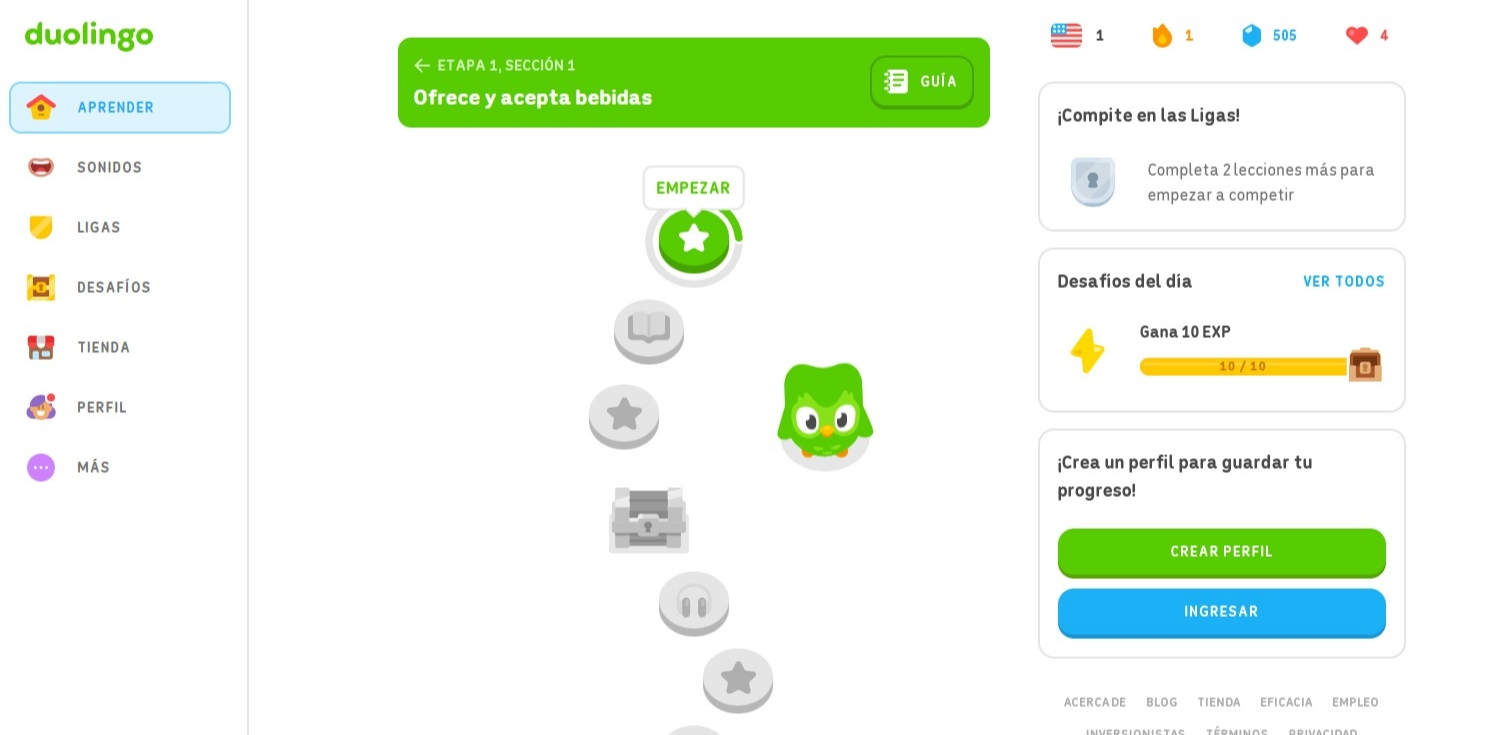
\includegraphics[width=0.48\textwidth]{figuras/duolingo_inicio.jpeg}
    \caption{Pantalla de inicio y menú principal de Duolingo.}
    \label{fig:duolingo1}
\end{figure}

\begin{figure}[htbp]
    \centering
    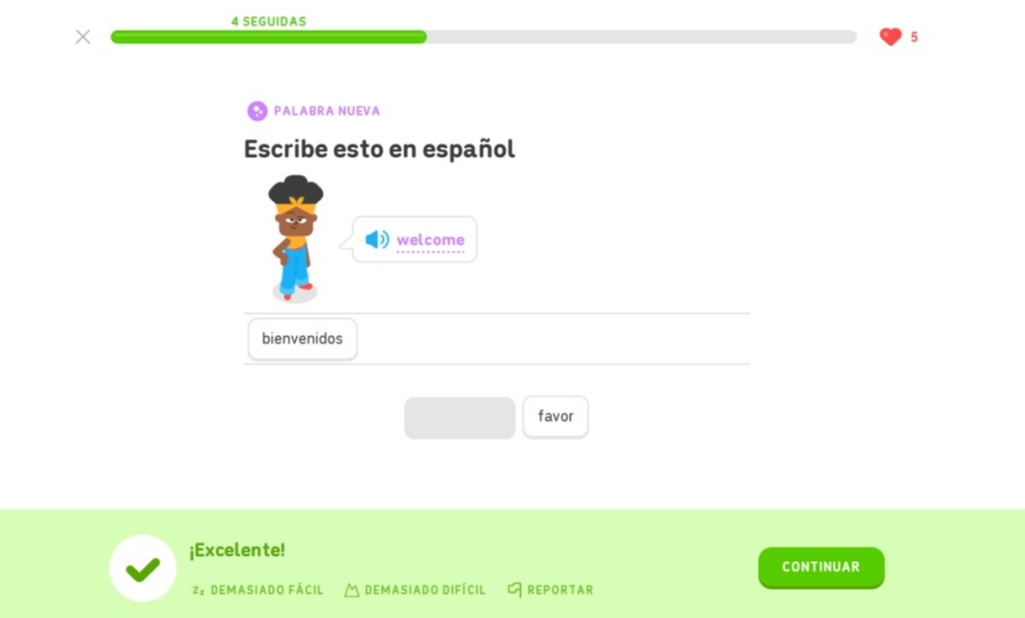
\includegraphics[width=0.48\textwidth]{figuras/duolingo_leccion.jpeg}
    \caption{Interfaz de resolución de ejercicios y conteo de corazones.}
    \label{fig:duolingo2}
\end{figure}

\begin{figure}[htbp]
    \centering
    
\includegraphics[width=0.48\textwidth]{figuras/duolingo_racha.jpeg}
    \caption{Panel de seguimiento de racha diaria y puntos XP.}
    \label{fig:duolingo3}
\end{figure}


\section{Tabla de Autoevaluación y Corrección}
En la Tabla \ref{tab:autoevaluacion} se presenta el proceso de autoevaluación donde se identificaron enunciados débiles o ambiguos (que incumplían la Cláusula 5.2.5 o 5.2.7) y se especifican sus versiones corregidas.

\begin{table}[htbp]
\centering
\caption{Autoevaluación de requisitos y versiones corregidas.}
\label{tab:autoevaluacion}
\small
\begin{tabularx}{\textwidth}{l X X X}
\toprule
\textbf{ID} & \textbf{Requisito Original (Deficiente)} & \textbf{Fallo Detectado (IEEE 29148)} & \textbf{Versión Corregida (Bien Formada)} \\
\midrule
RF-01 & La aplicación debe procesar los XP muy rápido para el usuario. & Uso de término ambiguo "muy rápido" (Cláusula 5.2.7). No es verificable. & El servidor backend debe procesar y registrar la puntuación XP en un tiempo menor o igual a 1.5 segundos. \\
\midrule
RF-02 & El sistema debe ser robusto y no caerse casi nunca durante la lección. & Uso de términos vagos "robusto" y "casi nunca" (Cláusula 5.2.7). & La aplicación móvil no debe presentar cierres imprevistos en más del 0.1\% de las sesiones activas. \\
\midrule
RF-04 & La pantalla inicial debe ser amigable e intuitiva para los estudiantes. & Término prohibido "amigable e intuitiva" (Cláusula 5.2.7). Incierto para probar. & El 95\% de los usuarios nuevos identificará el botón "Empezar Lección" en un tiempo menor a 4 segundos. \\
\midrule
RF-06 & El sistema restará vidas si te equivocas y te avisará al instante. & Falta de imperativo formal, lenguaje ambiguo ("al instante") y compuesto (5.2.5). & El sistema debe sustraer exactamente 1 corazón de la cuenta del usuario al confirmar una respuesta incorrecta. \\
\midrule
RD-10 & El servidor soportará bastantes usuarios simultáneos en la noche. & Ambigüedad en "bastantes usuarios" y falta de límites temporales claros (5.2.7). & La infraestructura debe procesar hasta 40,000 peticiones concurrentes por segundo entre las 18:00 y 22:00 UTC. \\
\bottomrule
\end{tabularx}
\end{table}

\section{Reflexión Personal}
Durante la realización de este trabajo, el tipo de requisito que representó un mayor nivel de dificultad para su formulación fue el de \textbf{Usabilidad / Calidad en Uso} bajo la norma ISO/IEC 25010:2023. 

La principal causa de esta dificultad radica en la tendencia habitual de definir la experiencia de usuario mediante adjetivos cualitativos y subjetivos tales como "interfaz intuitiva", "diseño atractivo" o "fácil navegación". La norma ISO/IEC/IEEE 29148:2018 prohíbe taxativamente este vocabulario en la Cláusula 5.2.7 debido a su falta de verificabilidad empírica. Transformar una percepción estética o de comodidad de uso en una métrica cuantitativa (por ejemplo, medir tasas de éxito de localización en segundos o porcentajes de usuarios en pruebas preliminares) requiere abstraer la interacción humana en parámetros observables y mensurables. Este ejercicio pone de manifiesto la importancia de la Ingeniería de Requisitos para cerrar la brecha entre los deseos imprecisos del usuario y las especificaciones técnicas rigurosas que necesita el equipo de software.

\section*{Declaración de Uso de Herramientas de Inteligencia Artificial}
Para el desarrollo de la presente tarea se utilizó el modelo de lenguaje AI Gemini (versión 2026) con el único propósito de estructurar la plantilla base de código LaTeX, revisar la ortografía en español y verificar la coherencia de compilación de las tablas. Todo el contenido conceptual, las métricas especificadas, las capturas de pantalla del sistema Duolingo y las reflexiones fueron revisados, redactados y validados de forma autónoma por el autor.


\bibliographystyle{IEEEtran}
\bibliography{referencias}

\end{document}
